\documentclass{standalone}
\usepackage{tikz}
\usetikzlibrary{patterns, positioning}


\begin{document}
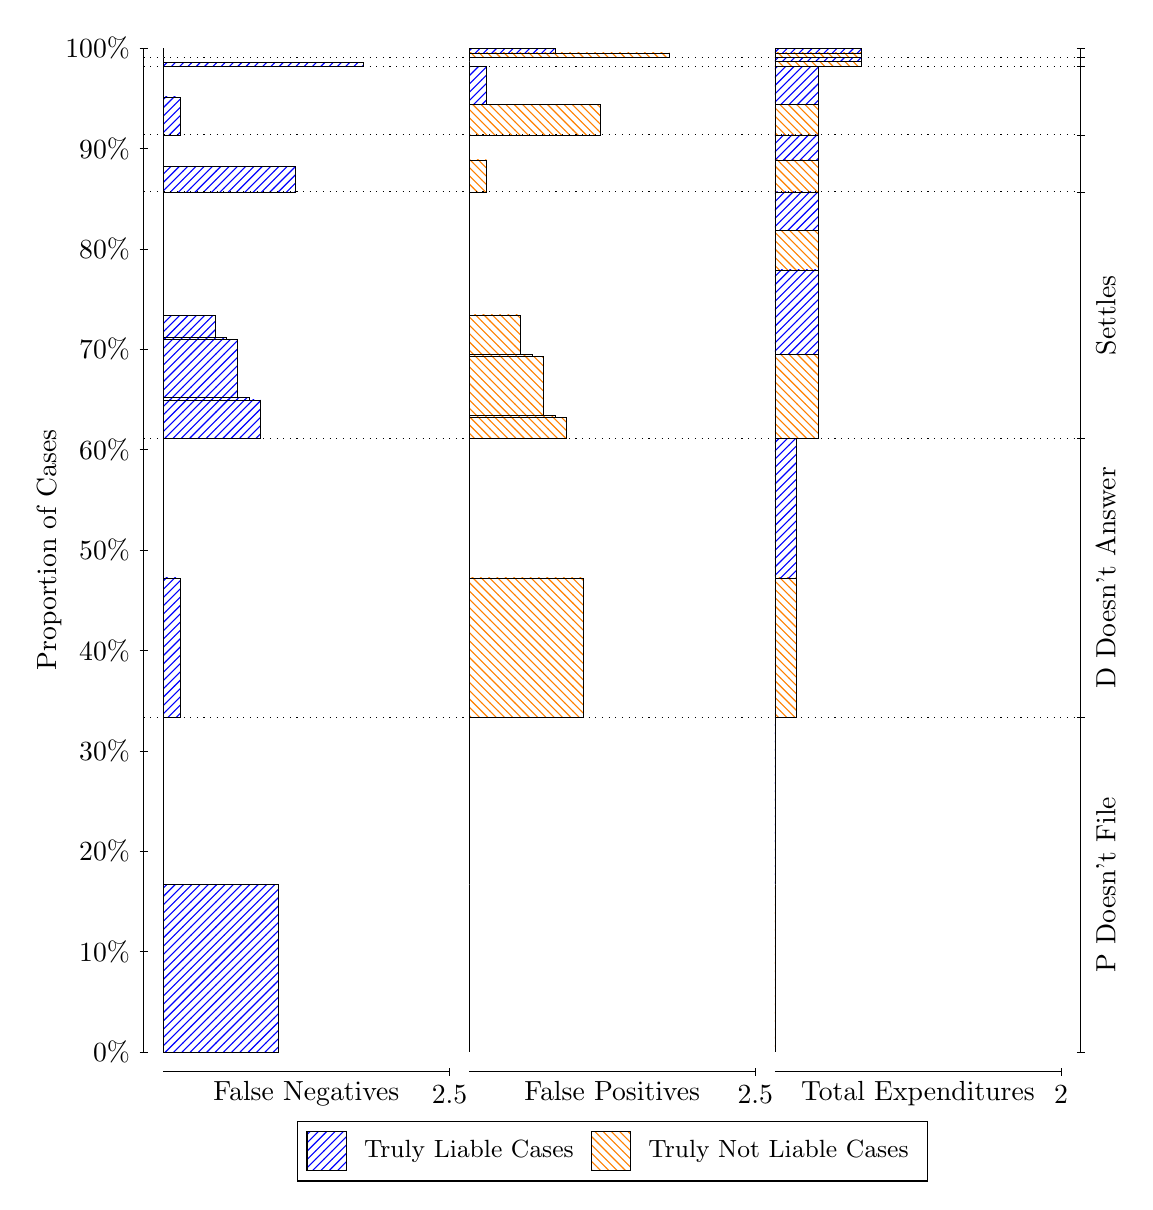
\begin{tikzpicture}
\draw[black, very thin] (1.5,1.75) -- (1.5,14.5);
\node[rotate=90, text=black, anchor=center] at (0.3, 8.125) {Proportion of Cases};
\draw[black, very thin] (1.45,1.75) -- (1.55,1.75);
\node[text=black, anchor=east] at (1.45, 1.75) {0\%};
\draw[black, very thin] (1.45,3.025) -- (1.55,3.025);
\node[text=black, anchor=east] at (1.45, 3.025) {10\%};
\draw[black, very thin] (1.45,4.3) -- (1.55,4.3);
\node[text=black, anchor=east] at (1.45, 4.3) {20\%};
\draw[black, very thin] (1.45,5.575) -- (1.55,5.575);
\node[text=black, anchor=east] at (1.45, 5.575) {30\%};
\draw[black, very thin] (1.45,6.85) -- (1.55,6.85);
\node[text=black, anchor=east] at (1.45, 6.85) {40\%};
\draw[black, very thin] (1.45,8.125) -- (1.55,8.125);
\node[text=black, anchor=east] at (1.45, 8.125) {50\%};
\draw[black, very thin] (1.45,9.4) -- (1.55,9.4);
\node[text=black, anchor=east] at (1.45, 9.4) {60\%};
\draw[black, very thin] (1.45,10.675) -- (1.55,10.675);
\node[text=black, anchor=east] at (1.45, 10.675) {70\%};
\draw[black, very thin] (1.45,11.95) -- (1.55,11.95);
\node[text=black, anchor=east] at (1.45, 11.95) {80\%};
\draw[black, very thin] (1.45,13.225) -- (1.55,13.225);
\node[text=black, anchor=east] at (1.45, 13.225) {90\%};
\draw[black, very thin] (1.45,14.5) -- (1.55,14.5);
\node[text=black, anchor=east] at (1.45, 14.5) {100\%};

\draw[black, very thin] (13.4,1.75) -- (13.4,14.5);
\draw[black, very thin] (13.35,1.75) -- (13.45,1.75);
\node[anchor=west] at (13.35, 1.75) {};
\draw[black, very thin] (13.35,6) -- (13.45,6);
\node[anchor=west] at (13.35, 6) {};
\draw[black, very thin] (13.35,9.5417) -- (13.45,9.5417);
\node[anchor=west] at (13.35, 9.5417) {};
\draw[black, very thin] (13.35,12.673) -- (13.45,12.673);
\node[anchor=west] at (13.35, 12.673) {};
\draw[black, very thin] (13.35,13.398) -- (13.45,13.398);
\node[anchor=west] at (13.35, 13.398) {};
\draw[black, very thin] (13.35,14.264) -- (13.45,14.264);
\node[anchor=west] at (13.35, 14.264) {};
\draw[black, very thin] (13.35,14.382) -- (13.45,14.382);
\node[anchor=west] at (13.35, 14.382) {};
\draw[black, very thin] (13.35,14.5) -- (13.45,14.5);
\node[anchor=west] at (13.35, 14.5) {};

\draw[black, very thin, pattern color=blue, pattern=north east lines] (1.75,1.75) rectangle (3.2033,3.875);
\draw[black, very thin, pattern color=orange, pattern=north west lines] (1.75,3.875) rectangle (1.75,6);
\draw[black, very thin, pattern color=blue, pattern=north east lines] (1.75,6) rectangle (1.968,7.7708);
\draw[black, very thin, pattern color=orange, pattern=north west lines] (1.75,7.7708) rectangle (1.75,9.5417);
\draw[black, very thin, pattern color=blue, pattern=north east lines] (1.75,9.5417) rectangle (2.9853,10.031);
\draw[black, very thin, pattern color=blue, pattern=north east lines] (1.75,10.031) rectangle (2.84,10.059);
\draw[black, very thin, pattern color=blue, pattern=north east lines] (1.75,10.059) rectangle (2.6947,10.804);
\draw[black, very thin, pattern color=blue, pattern=north east lines] (1.75,10.804) rectangle (2.5493,10.828);
\draw[black, very thin, pattern color=blue, pattern=north east lines] (1.75,10.828) rectangle (2.404,11.103);
\draw[black, very thin, pattern color=orange, pattern=north west lines] (1.75,11.103) rectangle (1.75,12.673);
\draw[black, very thin, pattern color=blue, pattern=north east lines] (1.75,12.673) rectangle (3.4213,12.993);
\draw[black, very thin, pattern color=orange, pattern=north west lines] (1.75,12.993) rectangle (1.75,13.398);
\draw[black, very thin, pattern color=blue, pattern=north east lines] (1.75,13.398) rectangle (1.968,13.879);
\draw[black, very thin, pattern color=orange, pattern=north west lines] (1.75,13.879) rectangle (1.75,14.264);
\draw[black, very thin, pattern color=blue, pattern=north east lines] (1.75,14.264) rectangle (4.2933,14.318);
\draw[black, very thin, pattern color=orange, pattern=north west lines] (1.75,14.318) rectangle (1.75,14.382);
\draw[black, very thin, pattern color=orange, pattern=north west lines] (1.75,14.382) rectangle (1.75,14.437);
\draw[black, very thin, pattern color=blue, pattern=north east lines] (1.75,14.437) rectangle (1.75,14.5);
\draw[black, very thin, pattern color=orange, pattern=north west lines] (5.6333,1.75) rectangle (5.6333,3.875);
\draw[black, very thin, pattern color=blue, pattern=north east lines] (5.6333,3.875) rectangle (5.6333,6);
\draw[black, very thin, pattern color=orange, pattern=north west lines] (5.6333,6) rectangle (7.0867,7.7708);
\draw[black, very thin, pattern color=blue, pattern=north east lines] (5.6333,7.7708) rectangle (5.6333,9.5417);
\draw[black, very thin, pattern color=orange, pattern=north west lines] (5.6333,9.5417) rectangle (6.8687,9.8099);
\draw[black, very thin, pattern color=orange, pattern=north west lines] (5.6333,9.8099) rectangle (6.7233,9.8379);
\draw[black, very thin, pattern color=orange, pattern=north west lines] (5.6333,9.8379) rectangle (6.578,10.586);
\draw[black, very thin, pattern color=orange, pattern=north west lines] (5.6333,10.586) rectangle (6.4327,10.61);
\draw[black, very thin, pattern color=orange, pattern=north west lines] (5.6333,10.61) rectangle (6.2873,11.111);
\draw[black, very thin, pattern color=blue, pattern=north east lines] (5.6333,11.111) rectangle (5.6333,12.673);
\draw[black, very thin, pattern color=orange, pattern=north west lines] (5.6333,12.673) rectangle (5.8513,13.078);
\draw[black, very thin, pattern color=blue, pattern=north east lines] (5.6333,13.078) rectangle (5.6333,13.398);
\draw[black, very thin, pattern color=orange, pattern=north west lines] (5.6333,13.398) rectangle (7.3047,13.783);
\draw[black, very thin, pattern color=blue, pattern=north east lines] (5.6333,13.783) rectangle (5.8513,14.264);
\draw[black, very thin, pattern color=orange, pattern=north west lines] (5.6333,14.264) rectangle (5.6333,14.328);
\draw[black, very thin, pattern color=blue, pattern=north east lines] (5.6333,14.328) rectangle (5.6333,14.382);
\draw[black, very thin, pattern color=orange, pattern=north west lines] (5.6333,14.382) rectangle (8.1767,14.437);
\draw[black, very thin, pattern color=blue, pattern=north east lines] (5.6333,14.437) rectangle (6.7233,14.5);
\draw[black, very thin, pattern color=orange, pattern=north west lines] (9.5167,1.75) rectangle (9.5167,3.875);
\draw[black, very thin, pattern color=blue, pattern=north east lines] (9.5167,3.875) rectangle (9.5167,6);
\draw[black, very thin, pattern color=orange, pattern=north west lines] (9.5167,6) rectangle (9.7892,7.7708);
\draw[black, very thin, pattern color=blue, pattern=north east lines] (9.5167,7.7708) rectangle (9.7892,9.5417);
\draw[black, very thin, pattern color=orange, pattern=north west lines] (9.5167,9.5417) rectangle (10.062,10.61);
\draw[black, very thin, pattern color=blue, pattern=north east lines] (9.5167,10.61) rectangle (10.062,11.682);
\draw[black, very thin, pattern color=orange, pattern=north west lines] (9.5167,11.682) rectangle (10.062,12.183);
\draw[black, very thin, pattern color=blue, pattern=north east lines] (9.5167,12.183) rectangle (10.062,12.673);
\draw[black, very thin, pattern color=orange, pattern=north west lines] (9.5167,12.673) rectangle (10.062,13.078);
\draw[black, very thin, pattern color=blue, pattern=north east lines] (9.5167,13.078) rectangle (10.062,13.398);
\draw[black, very thin, pattern color=orange, pattern=north west lines] (9.5167,13.398) rectangle (10.062,13.783);
\draw[black, very thin, pattern color=blue, pattern=north east lines] (9.5167,13.783) rectangle (10.062,14.264);
\draw[black, very thin, pattern color=orange, pattern=north west lines] (9.5167,14.264) rectangle (10.607,14.328);
\draw[black, very thin, pattern color=blue, pattern=north east lines] (9.5167,14.328) rectangle (10.607,14.382);
\draw[black, very thin, pattern color=orange, pattern=north west lines] (9.5167,14.382) rectangle (10.607,14.437);
\draw[black, very thin, pattern color=blue, pattern=north east lines] (9.5167,14.437) rectangle (10.607,14.5);
\draw[black, dotted] (1.5,6) -- (13.4,6);
\draw[black, dotted] (1.5,9.5417) -- (13.4,9.5417);
\draw[black, dotted] (1.5,12.673) -- (13.4,12.673);
\draw[black, dotted] (1.5,13.398) -- (13.4,13.398);
\draw[black, dotted] (1.5,14.264) -- (13.4,14.264);
\draw[black, dotted] (1.5,14.382) -- (13.4,14.382);
\draw[black, very thin] (1.75,1.5) -- (5.3833,1.5);
\node[text=black, anchor=north] at (3.5667, 1.5) {False Negatives};
\draw[black, very thin] (5.3833,1.45) -- (5.3833,1.55);
\node[text=black, anchor=north] at (5.3833, 1.45) {2.5};

\draw[black, very thin] (5.6333,1.5) -- (9.2667,1.5);
\node[text=black, anchor=north] at (7.45, 1.5) {False Positives};
\draw[black, very thin] (9.2667,1.45) -- (9.2667,1.55);
\node[text=black, anchor=north] at (9.2667, 1.45) {2.5};

\draw[black, very thin] (9.5167,1.5) -- (13.15,1.5);
\node[text=black, anchor=north] at (11.333, 1.5) {Total Expenditures};
\draw[black, very thin] (13.15,1.45) -- (13.15,1.55);
\node[text=black, anchor=north] at (13.15, 1.45) {2};

\node[text=black, centered, rotate=90] at (13.72, 3.875) {P Doesn't File};
\node[text=black, centered, rotate=90] at (13.72, 7.7708) {D Doesn't Answer};
\node[text=black, centered, rotate=90] at (13.72, 11.107) {Settles};





\draw (7.449999999999999,1.5) node[draw=none] (baseCoordinate) {};
\begin{scope}[align=center]
        \matrix[scale=0.5, draw=black, below=0.5cm of baseCoordinate, nodes={draw}, column sep=0.1cm]{
            \node[rectangle, draw, minimum width=0.5cm, minimum height=0.5cm, pattern color=blue, pattern=north east lines] {}; &
            \node[draw=none, font=\small, text=black] (B) {Truly Liable Cases}; &
            \node[rectangle, draw, minimum width=0.5cm, minimum height=0.5cm, pattern color=orange, pattern=north west lines] {}; &
            \node[draw=none, font=\small, text=black] (B) {Truly Not Liable Cases}; \\
            };
\end{scope}

\end{tikzpicture}
\end{document}